\documentclass[tikz,border=2pt]{standalone}
\usepackage{amsmath,amssymb}
\usepackage{pgfplots}
\pgfplotsset{compat=1.18}
\usetikzlibrary{arrows.meta}
\begin{document}
% Variance principle with alpha = 0.1 for X ~ Bernoulli(0.5) (Var X = 0.25), scaled to aX: the loading
% Pi(aX) - aE[X] = alpha a^2 Var(X) = 0.025 a^2 grows quadratically; at a = 2 it is 0.1, not 2(0.025) = 0.05.
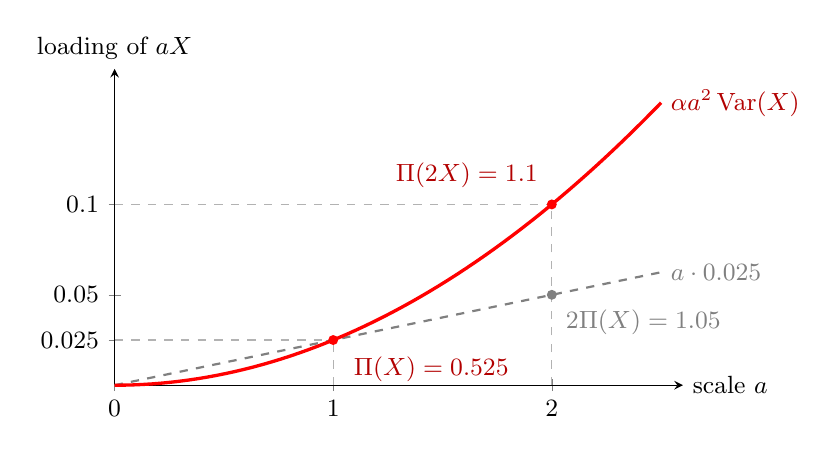
\begin{tikzpicture}[font=\small, >={Latex[length=2mm]}]
  \begin{axis}[
    axis lines=left, xmin=0, xmax=2.6, ymin=0, ymax=0.175,
    xtick={0,1,2}, ytick={0.025,0.05,0.1}, yticklabels={$0.025$,$0.05$,$0.1$},
    xlabel={scale $a$}, ylabel={loading of $aX$},
    xlabel style={at={(axis description cs:1,0)}, anchor=west},
    ylabel style={rotate=-90, at={(axis description cs:0,1)}, anchor=south},
    width=8.8cm, height=5.6cm, clip=false
    ]
    \addplot[gray, thick, dashed, domain=0:2.5, samples=2] {0.025*x};
    \node[gray, anchor=west] at (axis cs:2.5,0.0625) {$a\cdot0.025$};
    \addplot[red, very thick, domain=0:2.5, samples=60] {0.025*x^2};
    \node[red!70!black, anchor=west] at (axis cs:2.5,0.156) {$\alpha a^2\operatorname{Var}(X)$};
    \draw[gray!60, thin, dashed] (axis cs:1,0) -- (axis cs:1,0.025);
    \draw[gray!60, thin, dashed] (axis cs:2,0) -- (axis cs:2,0.1);
    \draw[gray!60, thin, dashed] (axis cs:0,0.1) -- (axis cs:2,0.1);
    \draw[gray!60, thin, dashed] (axis cs:0,0.025) -- (axis cs:1,0.025);
    \fill[red] (axis cs:1,0.025) circle (1.8pt);
    \fill[red] (axis cs:2,0.1) circle (1.8pt);
    \fill[gray] (axis cs:2,0.05) circle (1.8pt);
    \node[red!70!black, anchor=north west] at (axis cs:1.05,0.021) {$\Pi(X)=0.525$};
    \node[red!70!black, anchor=south east] at (axis cs:1.98,0.104) {$\Pi(2X)=1.1$};
    \node[gray, anchor=north west] at (axis cs:2.02,0.047) {$2\Pi(X)=1.05$};
  \end{axis}
\end{tikzpicture}
\end{document}
